\section{Beam Positioning}\label{sec:clas.beam}
%\FloatBarrier
There are several beam monitoring stations in hall \desg{b} before and after the \abbr{CLAS} detector (Fig.~\ref{fig:clas.beam.beforemonitors},Fig.~\ref{fig:clas.beam.aftermonitors}) to scan the important details of the electron beam prior to conversion into a photon beam and the details of the photon beam before and after entering into the target. Such quantities for the electron beam include position, intensity, dispersion, and current, while for the photon beam, position, dispersion and flux. Most of these monitoring stations  are used by the accelerator group to steer the beam to the target as they control all magnets that can substantially move the beam.
\begin{figure}[h!]\begin{center}
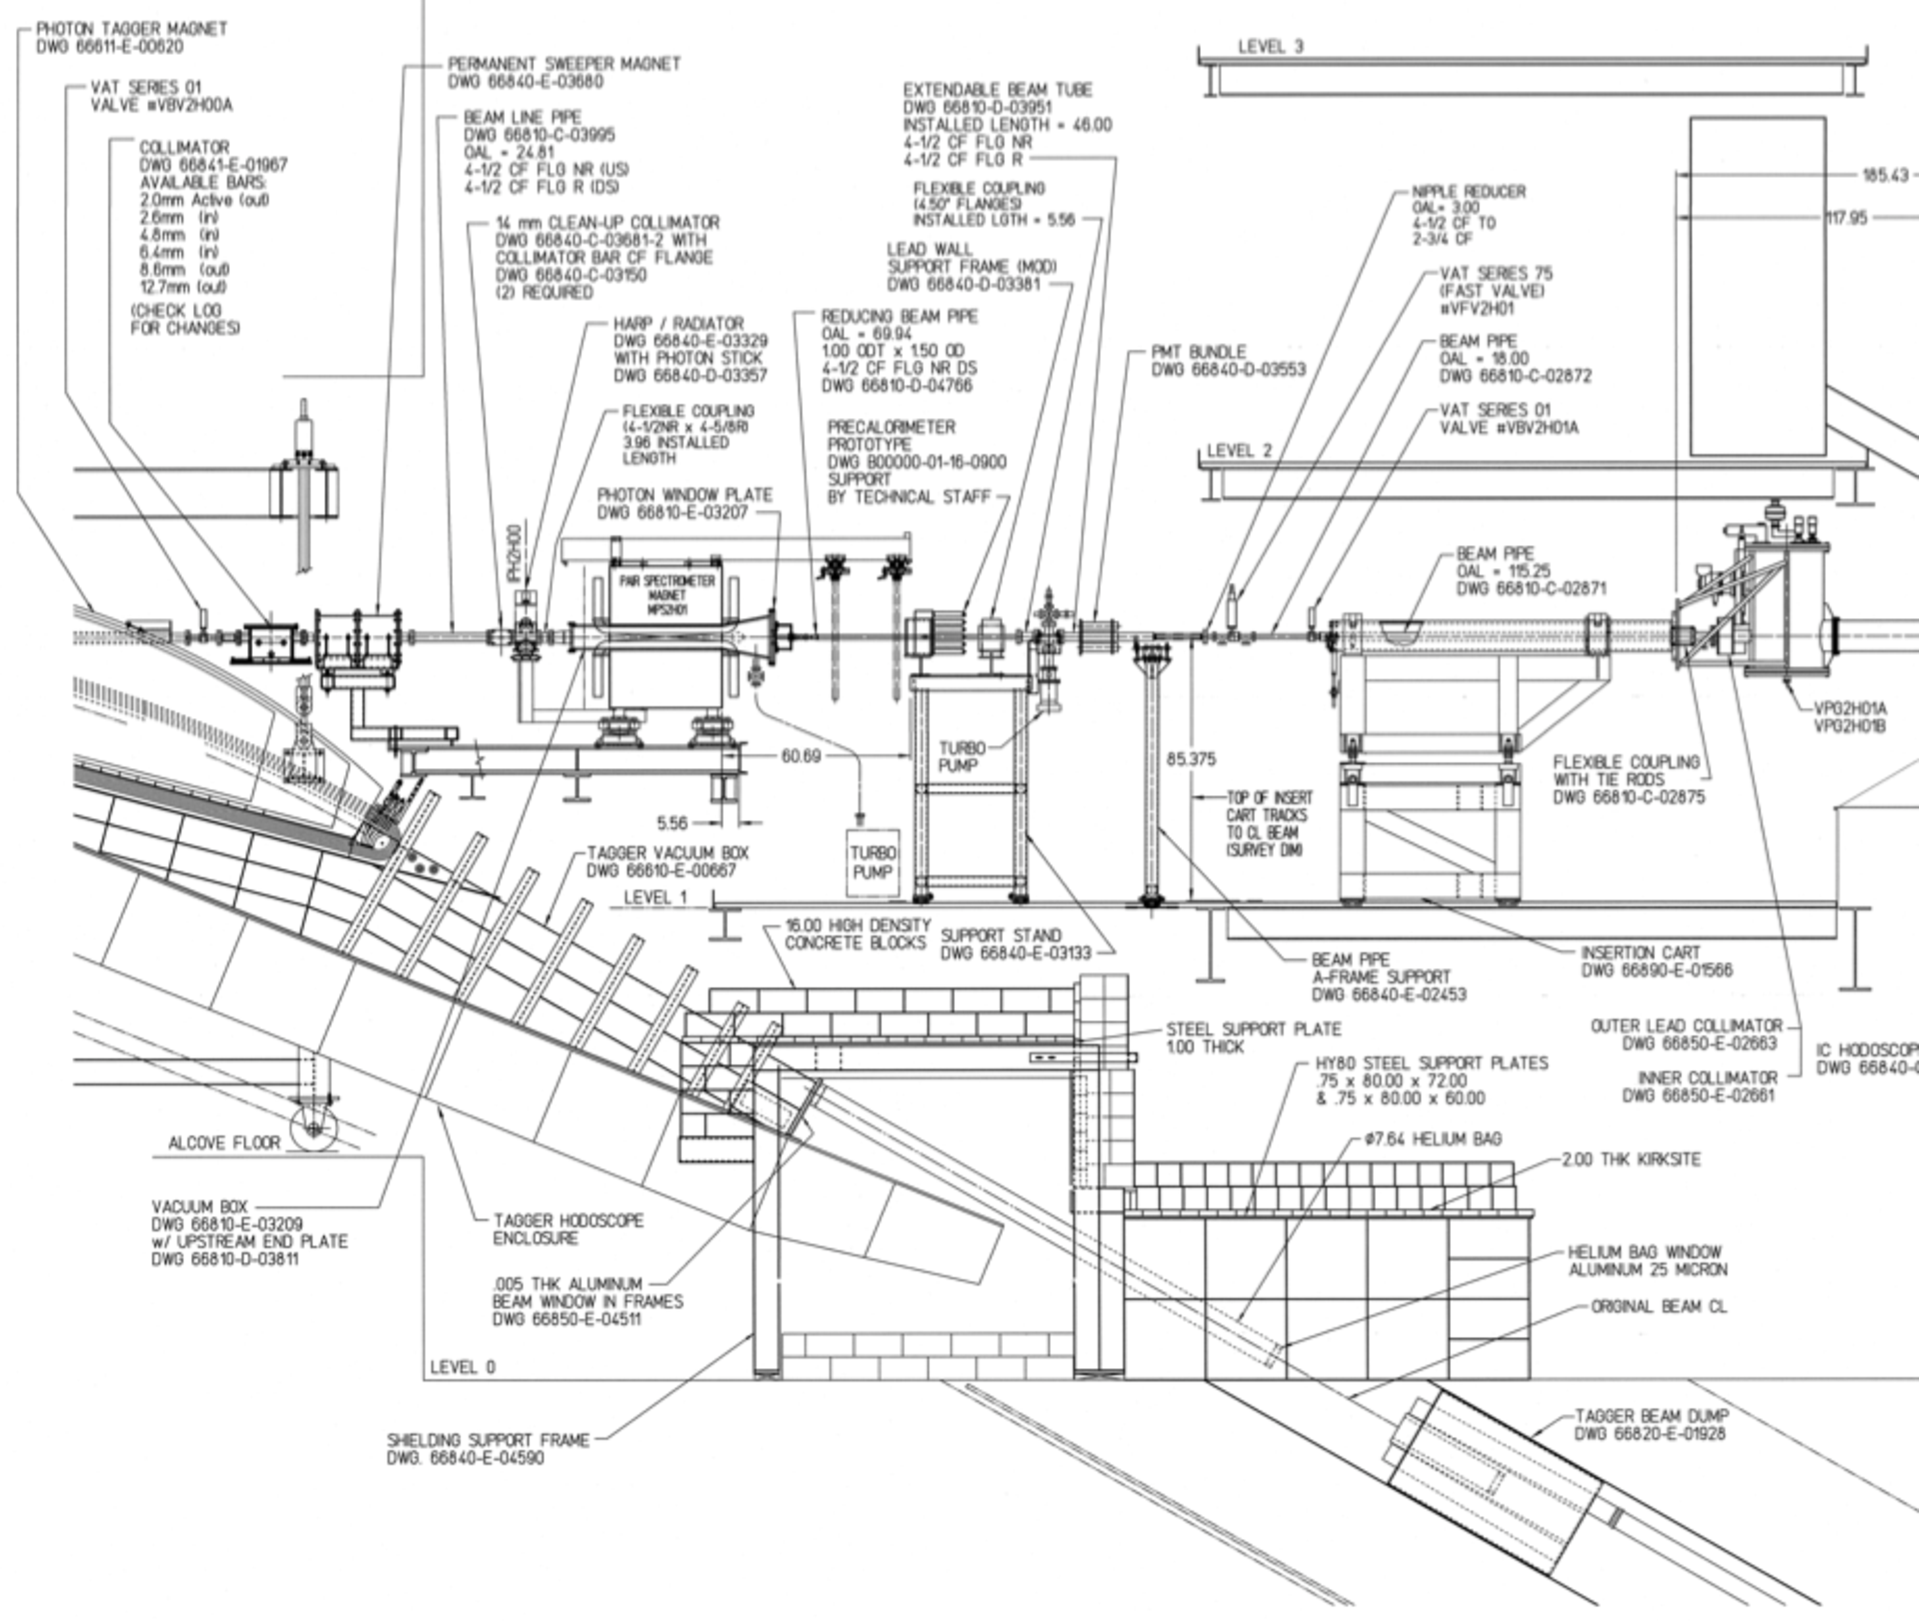
\includegraphics[width=\figwidth, height=\hfigheight]{\grpath/hall-b/G12_beam_blueprint.pdf}
\caption[Beamline and components of \g12 before target]{\label{fig:clas.beam.beforemonitors}{\coloronline}Beamline and components of \g12 before target}
\end{center}\end{figure}
There are two types of devices measure the beam position. The first type is represented by two beam position monitors (\abbr{BPM}s\label{abbr:bpm}) placed before the tagger. The position monitors use three radiofrequency cavities to measure the transverse location of the electron beam and its intensity. This information is used as feed back for the steering mechanism. The position monitors are noninvasive and measure at a rate of 1 Hz. 
The second type of device used to measure the beam position is the Harp Beam Profile Monitor, which also measures the electron beam dispersion. The harp devices consist of fine wires (20 and 50~{\um} W and 100~{\um} Fe) that pass through the beam at specific orientations and collect scattering electrons with a photomultiplier tube. This procedure obtains a horizontal ($x$) and vertical ($y$) profile of the electron beam and is required after any downtime or change in the beam. The accelerator group adjusts the beam position thus that more than 99\% of the collimated beam goes through the target volume. Since this process is invasive, it was only done when the drift-chambers and \abbr{DAQ} were turned off. The harp scan measurement for \g12 is shown in Fig.~\ref{fig:clas.beam.harpscan}, the width of the beam was contained within a 200 $\mathrm{\mu}$m diameter.



\begin{figure}\begin{center}
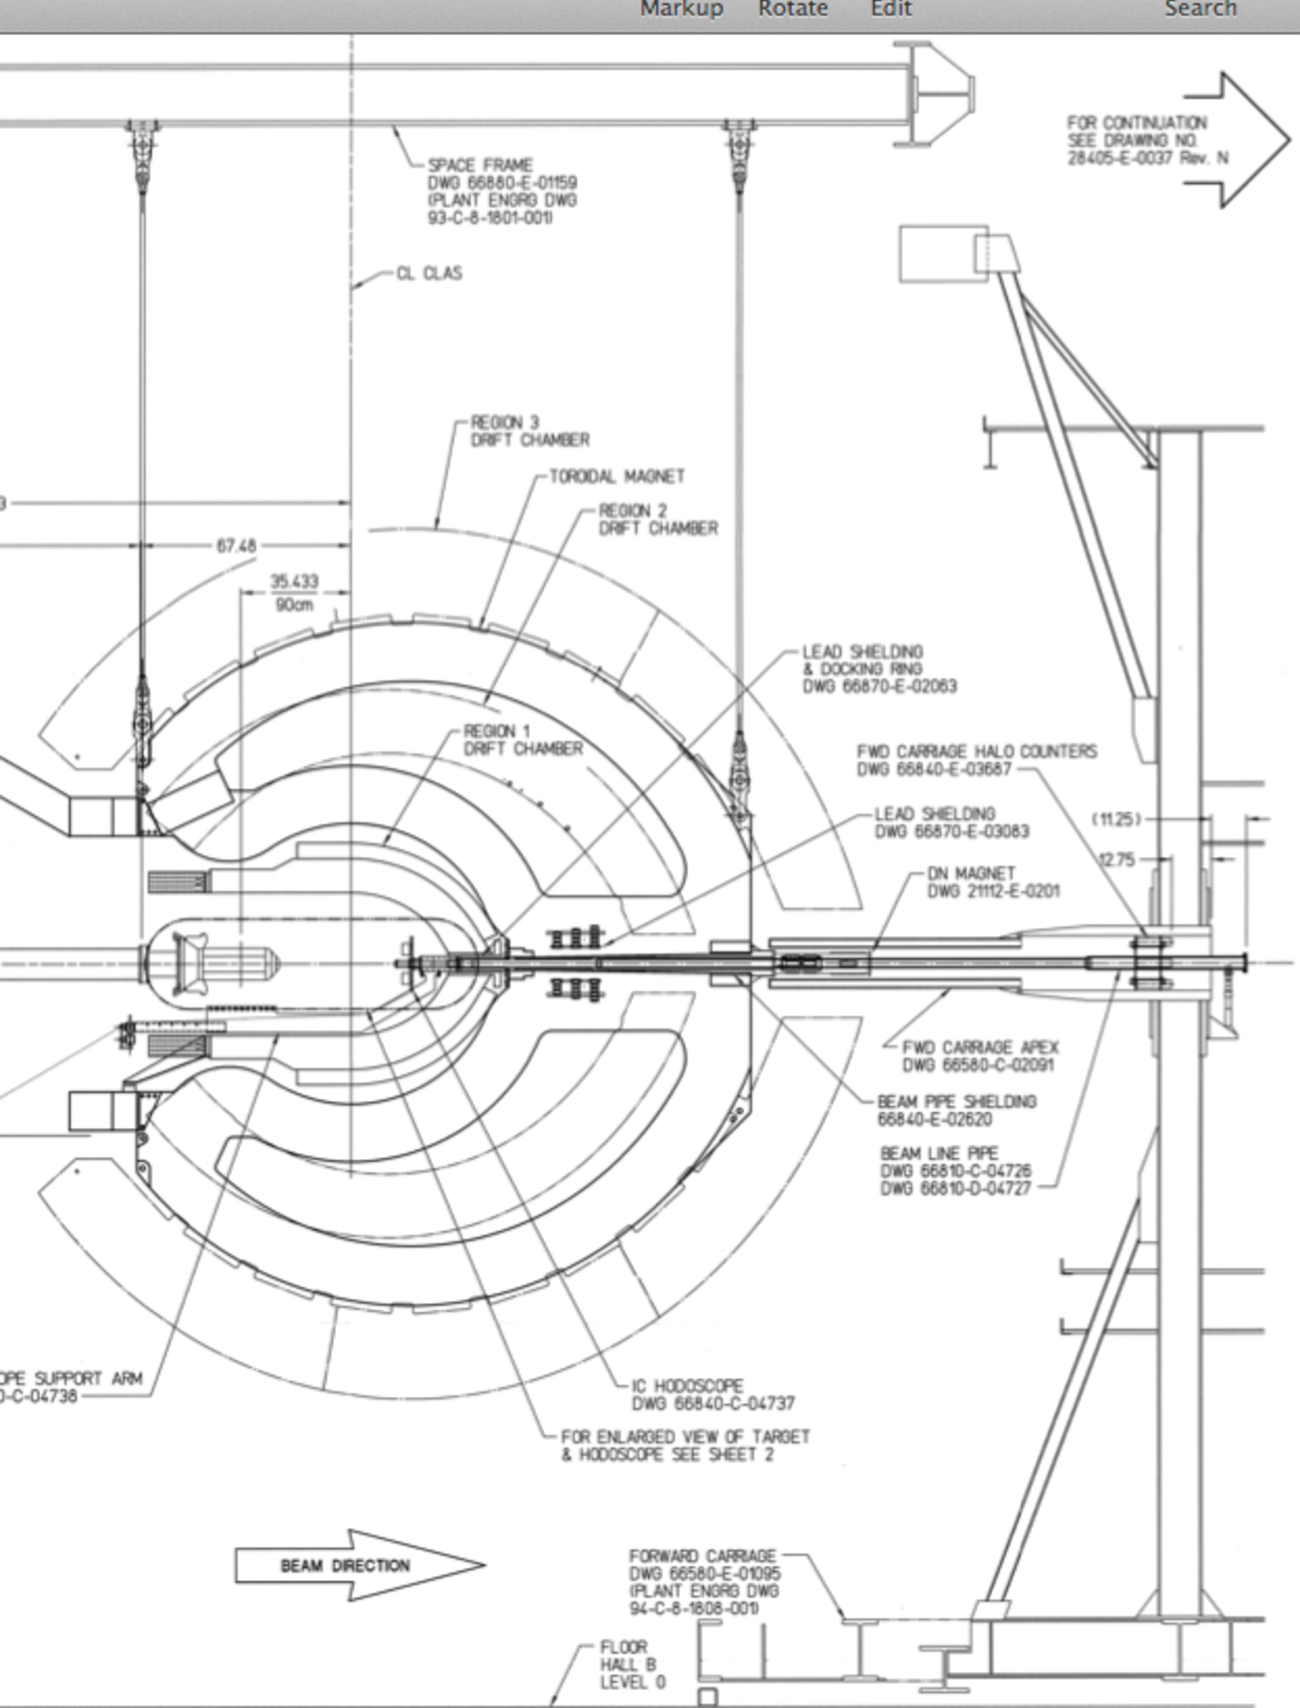
\includegraphics[width=\figwidth,height=\hfigheight]{\grpath/hall-b/G12_afterbeam_blueprint.pdf}
\caption[Beamline and \abbr{CLAS} components in \g12]{\label{fig:clas.beam.aftermonitors}{\coloronline}Beamline and \abbr{CLAS} components in \g12}
\end{center}\end{figure}

\begin{figure}\begin{center}
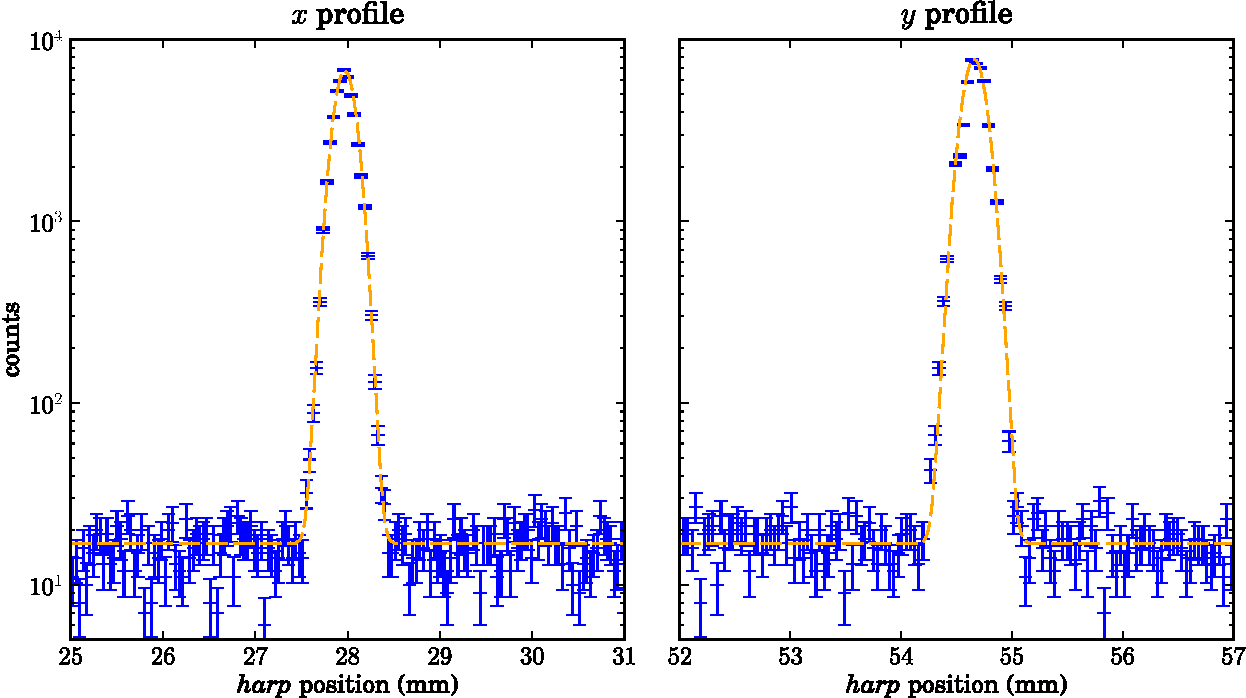
\includegraphics[width=\figwidth,height=\qfigheight]{\grpath/calibration/harpscan.pdf}
\caption[Example \emph{harp} Scan for \g12]{\label{fig:clas.beam.harpscan}{\coloronline}A typical \emph{harp} scan done just prior to run 56426. Shown are the $x$ and $y$ profiles of the electron beam just before the tagger. The dashed orange line is a Gaussian fit to the data: $\sigma_x~=~0.115$~mm and $\sigma_y~=~0.105$~mm.}
\end{center}\end{figure}

The Total Absorption Shower Counter, seen in Fig.~\ref{fig:clas.beam.afterCLAS}, located downstream of \abbr{CLAS}, measures the photon flux. The \abbr{TASC}, consists of four lead glass blocks of $\sim$ 17 radiation lengths, each coupled to a photo-multiplier tube (\abbr{PMT}\label{abbr:pmt}). The \abbr{TASC} is approximately 100\% efficient at detecting photons at beam currents less that 100~pA\cite{clas.tagger,clas.tagger.calib}. Since \g12 was 65~nA, special low current normalization runs of current (50~pA, see Table~\ref{tab:data.calibruns}) were taken several times throughout \g12. The ratio of electrons with hits in the left and right \abbr{TDC} matching in time and a corresponding hit in an E-counter(Sec.~\ref{sec:clas.tagr}) to that of photons detected in the \abbr{TASC} gives the tagging ratio used to calibrate the tagger and measure the flux throughout the entire \g12 run period.

\begin{figure}[h!]\begin{center}
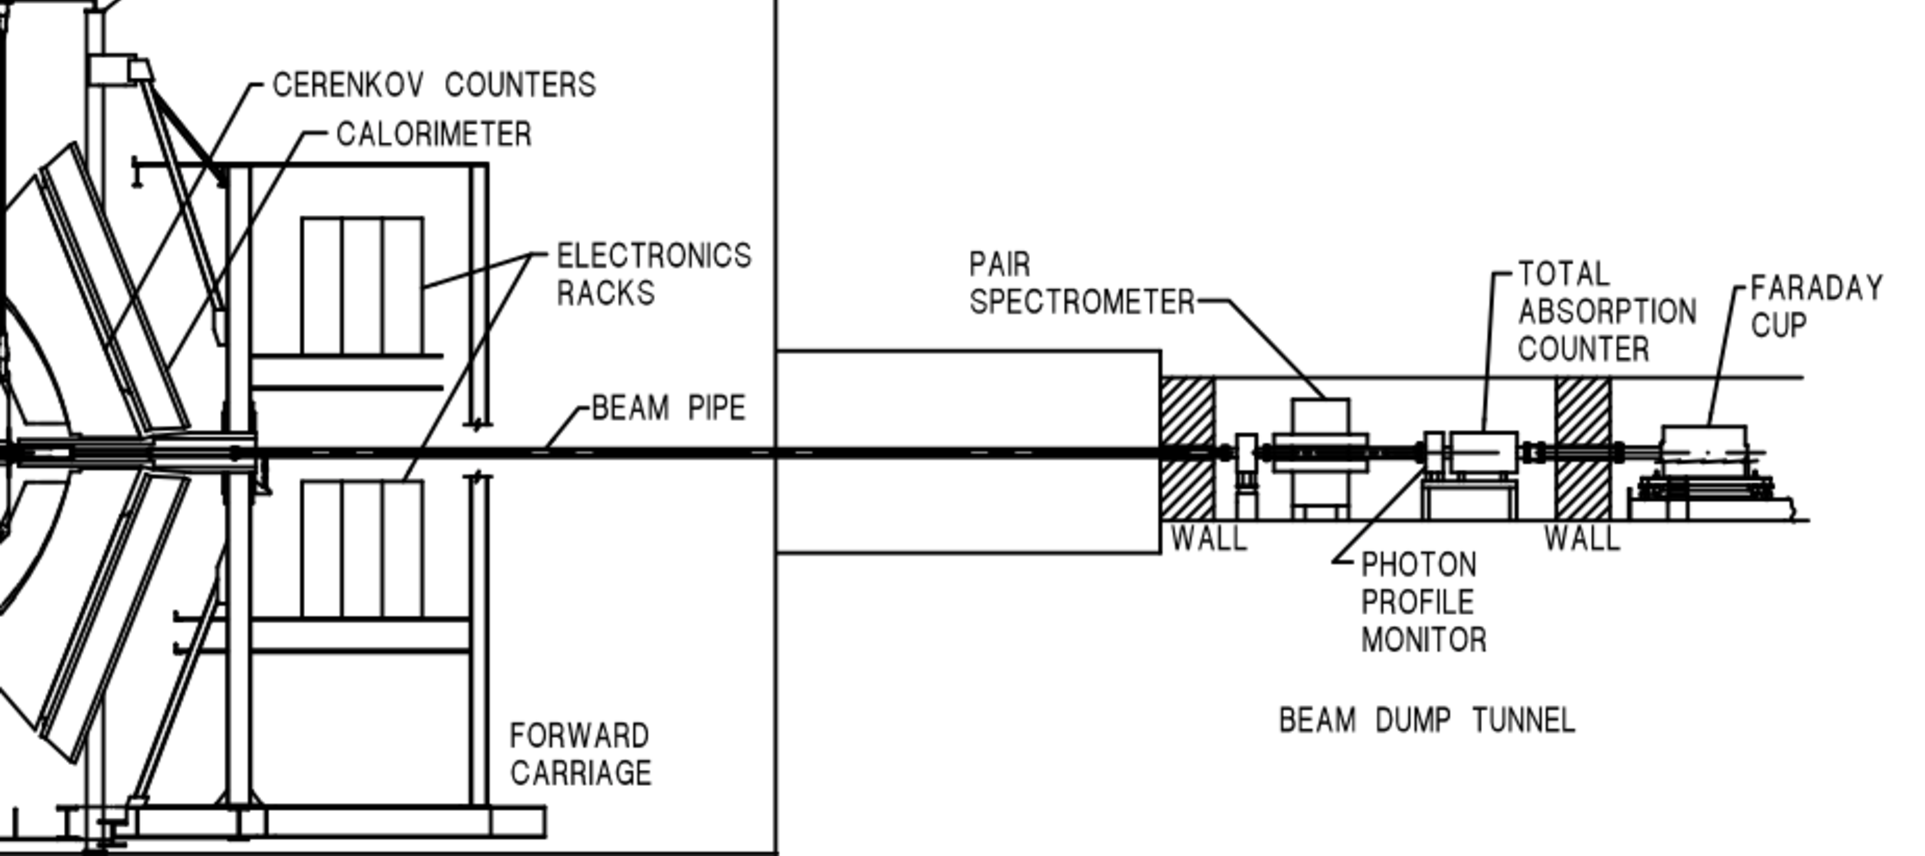
\includegraphics[width=\figwidth,height=0.8\qfigheight]{\grpath/hall-b/TASC_blueprint.pdf}
\caption[Beamline and components after \abbr{CLAS} ]{\label{fig:clas.beam.afterCLAS}{\coloronline}Beamline components in \g12 after \abbr{CLAS}}
\end{center}\end{figure}

\FloatBarrier